%%%%%%%%%%%%%%%%%%%%%%%%%%%%%%%%%%%%%%%%%%%%%%%%%%%%%%%%%%%%%%%%%
% elastic.tex
% Authors: Vladimir Ivantchenko, Vladimir Grichine, Dennis Wright
%%%%%%%%%%%%%%%%%%%%%%%%%%%%%%%%%%%%%%%%%%%%%%%%%%%%%%%%%%%%%%%%%
\paragraph{Elastic scattering models}
Four options exist in \Gfour{} for the simulation of elastic hadron scattering
from nuclei: the GHEISHA-based and CHIPS-based parameterized models,
the Glauber approach, and diffuse diffraction.

The GHEISHA-based models (\gclass{G4HadronElastic}) \cite{hadbib:gheisha} are
valid for all long-lived hadrons at all incident energies.  They sample the 
momentum transfer from a sum of exponentials whose amplitudes are parameterized
in $Z$, $A$ and incident momentum.  These models are fast, but significantly 
overshoot the data at large angles.

The CHIPS-based models (\gclass{G4ChipsElasticModel}) \cite{hadbib:CHIPS} are
similar, but sample the momentum transfer from a more complex parameterization
which includes details of the nuclear size and potential.  Hence, features like 
diffraction minima are represented.  This model is valid for incident protons,
neutrons, pions, kaons and anti-protons at all energies.

The \gclass{G4ElasticHadrNucleusHE} model depends on Glauber multiple scattering
\cite{hadbib:glauber70} in a nucleus which is described by its impact parameter 
profile.  The energy dependence of the scattering is largely determined by a 
phenomenological combination of hadron-nucleon cross sections.  The model is
valid for all long-lived hadrons of energies greater than 1 GeV.

The \gclass{G4DiffuseElastic} model \cite{hadbib:difel} uses an optical model
of the nucleus and takes into account the diffuse nuclear halo as well as Coulomb 
effects.  It is valid for incident protons, neutrons, pions and kaons of all 
energies.    

The four models are compared to data for 1 GeV protons on silicon in 
Figure~\ref{pSiT1GeVmodsum}.

\begin{figure}
% \centering \includegraphics[height=3.3in,width=3.6in]{figures/pSiT1GeVmodsum.eps}
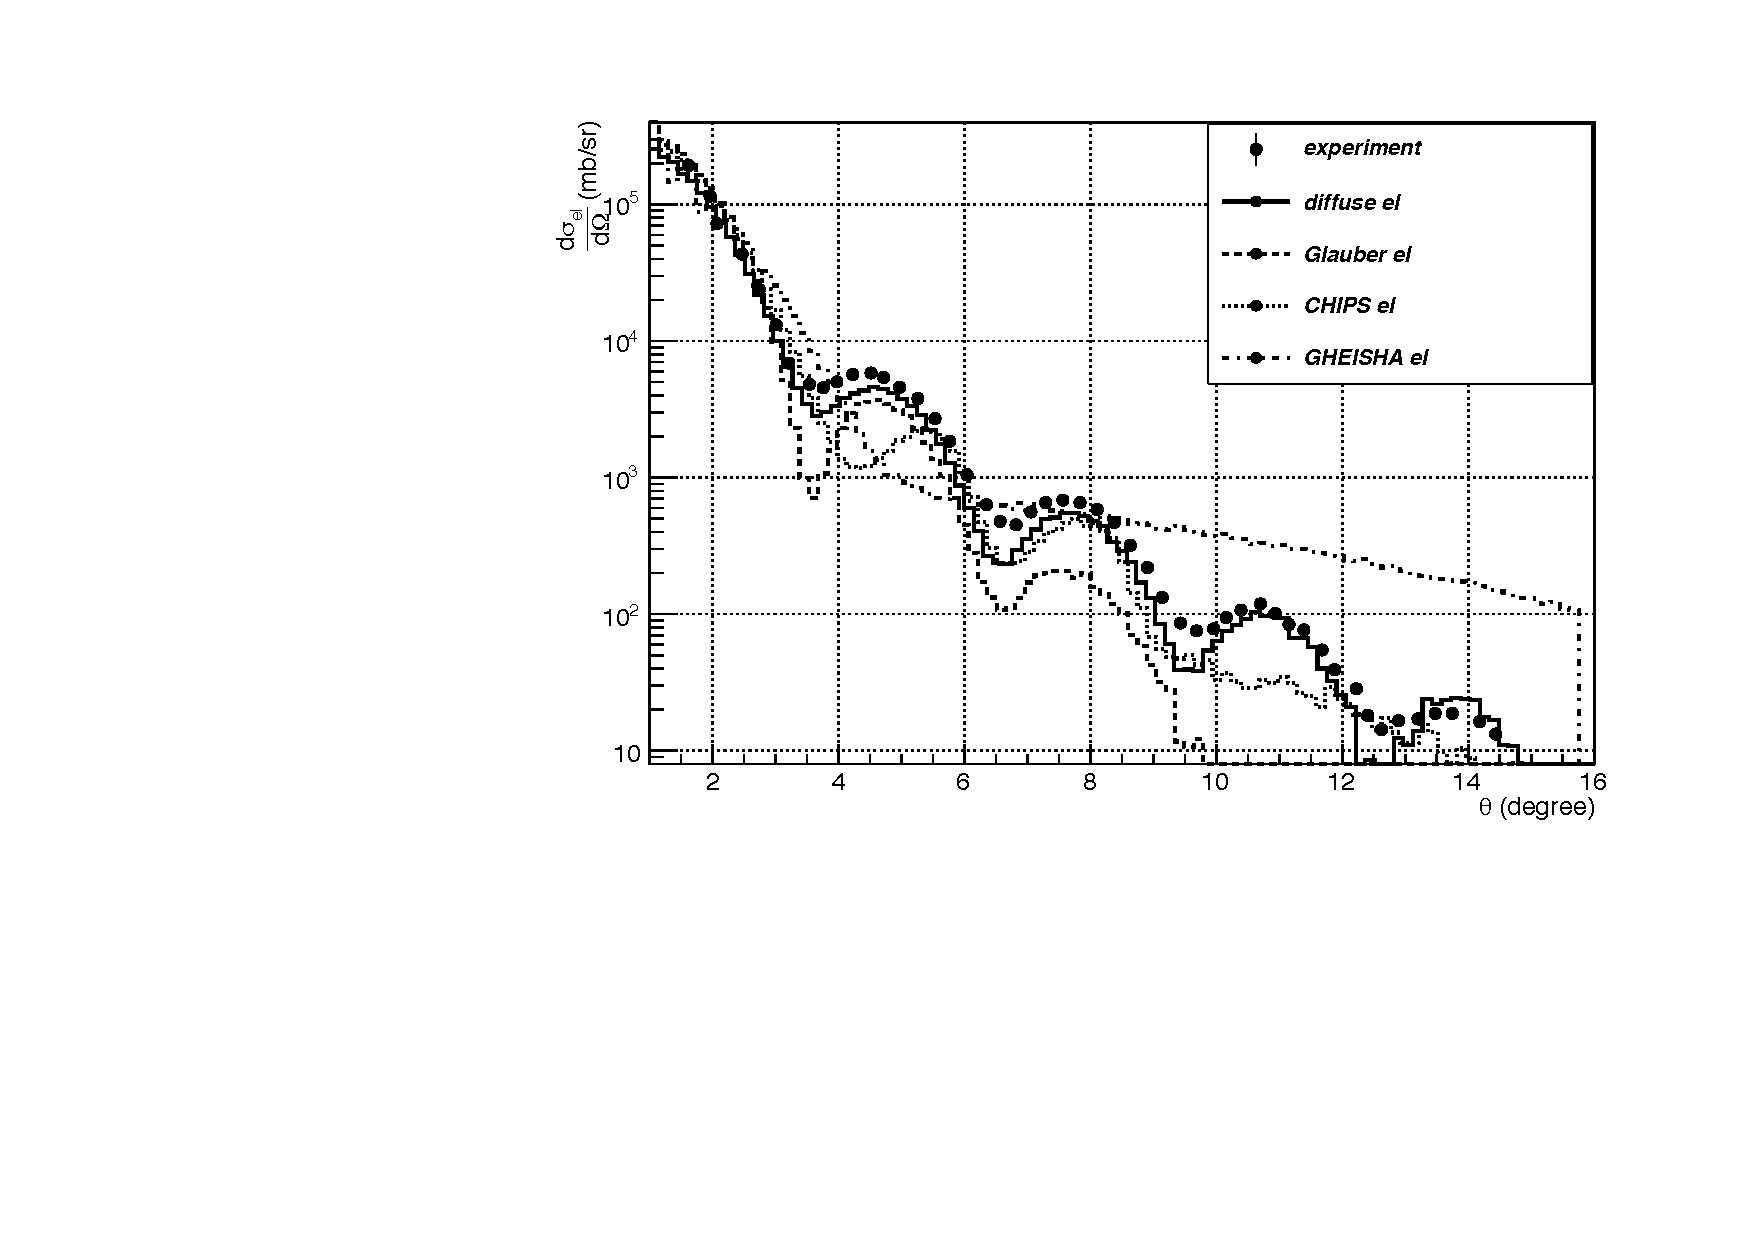
\includegraphics[width=0.5\textwidth]{figures/pSiT1GeVmodsum.pdf}
\caption{Differential elastic scattering cross sections for 1 GeV protons on 
         silicon versus polar scattering angle.  The histograms represent the 
         diffuse, Glauber, CHIPS and GHEISHA models. The solid circles are 
         experimental data~\cite{hadbib:alkh78}.}
\label{pSiT1GeVmodsum}
\end{figure}


